\section{Applying these tools to advance microbiome science}\label{section_contributions}

Sections~\ref{section_book} and~\ref{section_bottlenecks} presented my work
on standardizing and improving the pipelines to analyze microbial community data.
Sections~\ref{subsection_komodo},~\ref{subsection_emp},~\ref{subsection_ag}
and~\ref{subsection_bloom} provide examples of manuscripts that I have been
involved in that have taken advantage of my work presented so far.

Section~\ref{subsection_komodo} has been adapted from the original publication in
``The oral and skin microbiomes of captive Komodo dragons are significantly shared
with their habitat''. E.R. Hyde, J. A. Navas-Molina, S. J. Song, J. G. Kueneman,
G. Ackermann, C. Cardona, G. Humphrey, D. Boyer, T. Weaver, J. R. Mendelson,
V. J. McKenzie, J. A. Gilbert, R. Knight \emph{mSystems}, 2016. DOI: 10.1128/mSystems.00046-16

Section~\ref{subsection_emp} has been adapted from the original publication in
``A communal catalogue reveals Earth's multiscale microbial diversity''.
\emph{Nature} L. R. Thompson, J. G. Sanders, D. McDonald, A. Amir,
J. Ladau, K. J. Locey, R. J. Prill, A. Tripathi, S. M. Gibbons, G. Ackermann,
J. A. Navas-Molina, S. Janssen, E. Kopylova, Y. Vazquez-Baeza, A. Gonzalez,
J. T. Morton, S. Mirarab, Z. Z. Xu, L. Jiang, M. F. Haroon, J. Kanbar, Q. Zhu,
S. J. Song, T. Kosciolek, N. A. Bokulich, J. Lefler, C. J. Brislawn, G. Humphrey,
S. M. Owens, J. Hampton-Marcell, D. Berg-Lyons, V. McKenzie, N. Fierer, J. A. Fuhrman,
A. Clauset, R. L. Stevens, A. Shade, K. S. Pollard, K. D. Goodwin, J. K. Jansson,
J. A. Gilbert, R. Knight, The Earth Microbiome Project Consortium, 2017. DOI: 10.0.4.14/nature24621

Section~\ref{subsection_ag}, in part, has been submitted for publication of the
material as it may appear in Science, 2018, D. McDonald, E. R. Hyde, J. W. Debelius,
J. T. Morton, A. Gonzalez, G. Ackermann, A. A. Aksenov, B. Behsaz, C. Brennan,
Y. Chen, L. DeRight Goldasich, P. C. Dorrestein, R. R. Dunn, A. K. Fahimipour,
J. Gaffney, J. A Gilbert, G. Gogul, J. L. Green, P. Hugenholtz, G. Humphrey,
C. Huttenhower, M. A. Jackson, S. Janssen, D. V. Jeste, L. Jiang, S. T. Kelley,
D. Knights, T. Kosciolek, J. Ladau, J. Leach, C. Marotz, D. Meleshko, A. V. Melnik,
J. L. Metcalf, H. Mohimani, E. Montassier, J. A. Navas-Molina, T. T. Nguyen,
S. Peddada, P. Pevzner, K. S. Pollard, G. Rahnavard, A. Robbins-Pianka,
N. Sangwan, J. Shorenstein, L. Smarr, S. J. Song, T. Spector, A. D. Swafford,
V. G. Thackray, L. R. Thompson, Y. Vazquez-Baeza, A. Vrbanac, P. Wischmeyer,
E. Wolfe, Q. Zhu, The American Gut Consortium, R. Knight.

Section~\ref{subsection_bloom} has been adapted from the original publication in
``Correcting for microbial blooms in fecal samples during room-temperature shipping''.
\emph{mSystems} A. Amir, D. McDonald, J. A. Navas-Molina, J. Debelius, J. T. Morton,
E. R. Hyde, A. Robbins-Pianka, R. Knight 2017. DOI: 10.1128/mSystems.00199-16

\subsection{The oral and skin microbiomes of captive Komodo dragons are significantly shared with their habitat}\label{subsection_komodo}

The following text has been adapted from the original publication in
\textsl{mSystems, 16}. As a contributor to this manuscript, I performed the data
analysis included in the manuscript, wrote the IPython notebok \cite{Perez2007}
attached to the publication, generated figures and reviewed drafts of the manuscript.

The evidence for both vertebrate animals and humans indicates that closed
environments not only limit exposure to complex microbial diversity but also
promote microbial transfer from the host to the environment, rather than from
the environment to the host. Fully characterizing the effects of captivity on
host-environment microbial sharing will be key for future studies of vertebrate
microbial ecology and may prove instrumental in improving animal husbandry
practices. To more thoroughly describe the effects of captivity on host-environment
microbiome sharing and how this may affect vertebrate ecology studies, there is a
need to examine the microbial ecology of the host-environment interaction in a
number of vertebrate species, both in the wild and in captivity. Here we use as
a model the captive Komodo dragon (\emph{Varanus komodoensis}), applying 16S \gls{rrna}
amplicon sequencing to characterize the oral, fecal, skin, and environment-associated
microbiomes to answer two main questions: first, is the extent of host-environment
microbiome sharing observed for captive Komodo dragons typical of that observed
among other vertebrates living in closed environments, and second, is the
host-environment microbiome sharing observed among captive Komodo dragons
characteristically different from that observed among wild vertebrates? To
answer these questions, we explored whether host-environment microbiome sharing
in captive Komodo dragons was similar to the pattern observed for humans and pets
living in homes \cite{Lax2014} and dissimilar to the pattern observed among wild amphibians
living in open ecosystems \cite{Kueneman2014}. Together with existing studies, the data suggest that
living in closed environments is associated with extensive host-environment microbial
sharing. This sharing is likely to be circular in nature—the host contributes
microbes to its environment and then, in the absence of significant exposure to
microbes from external sources, reacquires those microbes from its environment,
only to share them with the environment once again (or vice versa). This may be
a radical departure from the microbial communities and exposures which vertebrates
cohabitate with and have evolved alongside in the wild, and could have significant
effects on health and disease \cite{Lax2015}.

To determine how much of the Komodo dragon's microbiome is shared with its environment
(or vice versa) and whether and how specific the environment is to the dragon, we
obtained matched dragon-environment samples from the Denver and Honolulu zoos. In
terms of taxonomic composition and abundance, environmental microbiomes appeared most
similar to salivary and skin microbiomes from the phylum down to the genus level
in both the Denver and Honolulu zoo cohorts (see Figure~\ref{KomodoST} A).

We applied SourceTracker \cite{Knights2011} to samples from the Denver Zoo Komodo
dragons to determine which dragon microbiome sources (saliva, feces, and skin)
contributed to the dragon environment. The microbiomes of items in the Denver
Komodo dragons’ enclosures were largely sourced from Komodo dragon salivary, skin,
and fecal samples (Figure~\ref{KomodoST} B), with unknown sources comprising less
than 50\% of the microbial communities of most environmental sample types.
Additionally, skin, saliva, and fecal communities were distinct from one another
in a SourceTracker independence test (Figure~\ref{KomodoST} B), suggesting that
any skin, saliva, or fecal communities detected on environmental materials actually
came from the dragon’s skin, mouth, or feces. Further supporting this point—at
least in the context of saliva—several bacterial taxa found in the mouths of the
Komodo dragons studied here, including \emph{Staphylococcus}, \emph{Corynebacterium},
\emph{Pseudomonas}, and \emph{Bacteroides}, have previously been reported in the
mouths of captive Komodo dragons \cite{Montgomery2002, Goldstein2013}. This
suggests that environmental microbes designated as sourced from the Komodo dragon’s
oral cavity likely actually do come from the mouth and not any other source. The
nature and extent of host-microbiome transfer to environmental objects varied with
sample type; for example, Komodo dragon saliva was the main source of the microbial
communities detected in soil and on rock and glass, while Komodo dragon skin was
the main source of the microbial communities detected on metal (Figure~\ref{KomodoST} B).
Performing SourceTracker analyses with Komodo dragon samples designated as sinks
and environmental samples designated as sources revealed that the microbial
communities of Komodo dragon fecal, saliva, and skin samples are sourced from a
variety of environmental materials, each contributing 30\% or less of the microbial community
(Figure~\ref{KomodoST} C and D). There is no one environmental material that contributes
more than any other material to Komodo dragon feces or saliva; however, Komodo skin microbial
communities are sourced majorly from glass and unknown sources (each ~40\%).

\begin{figure}[htbp]
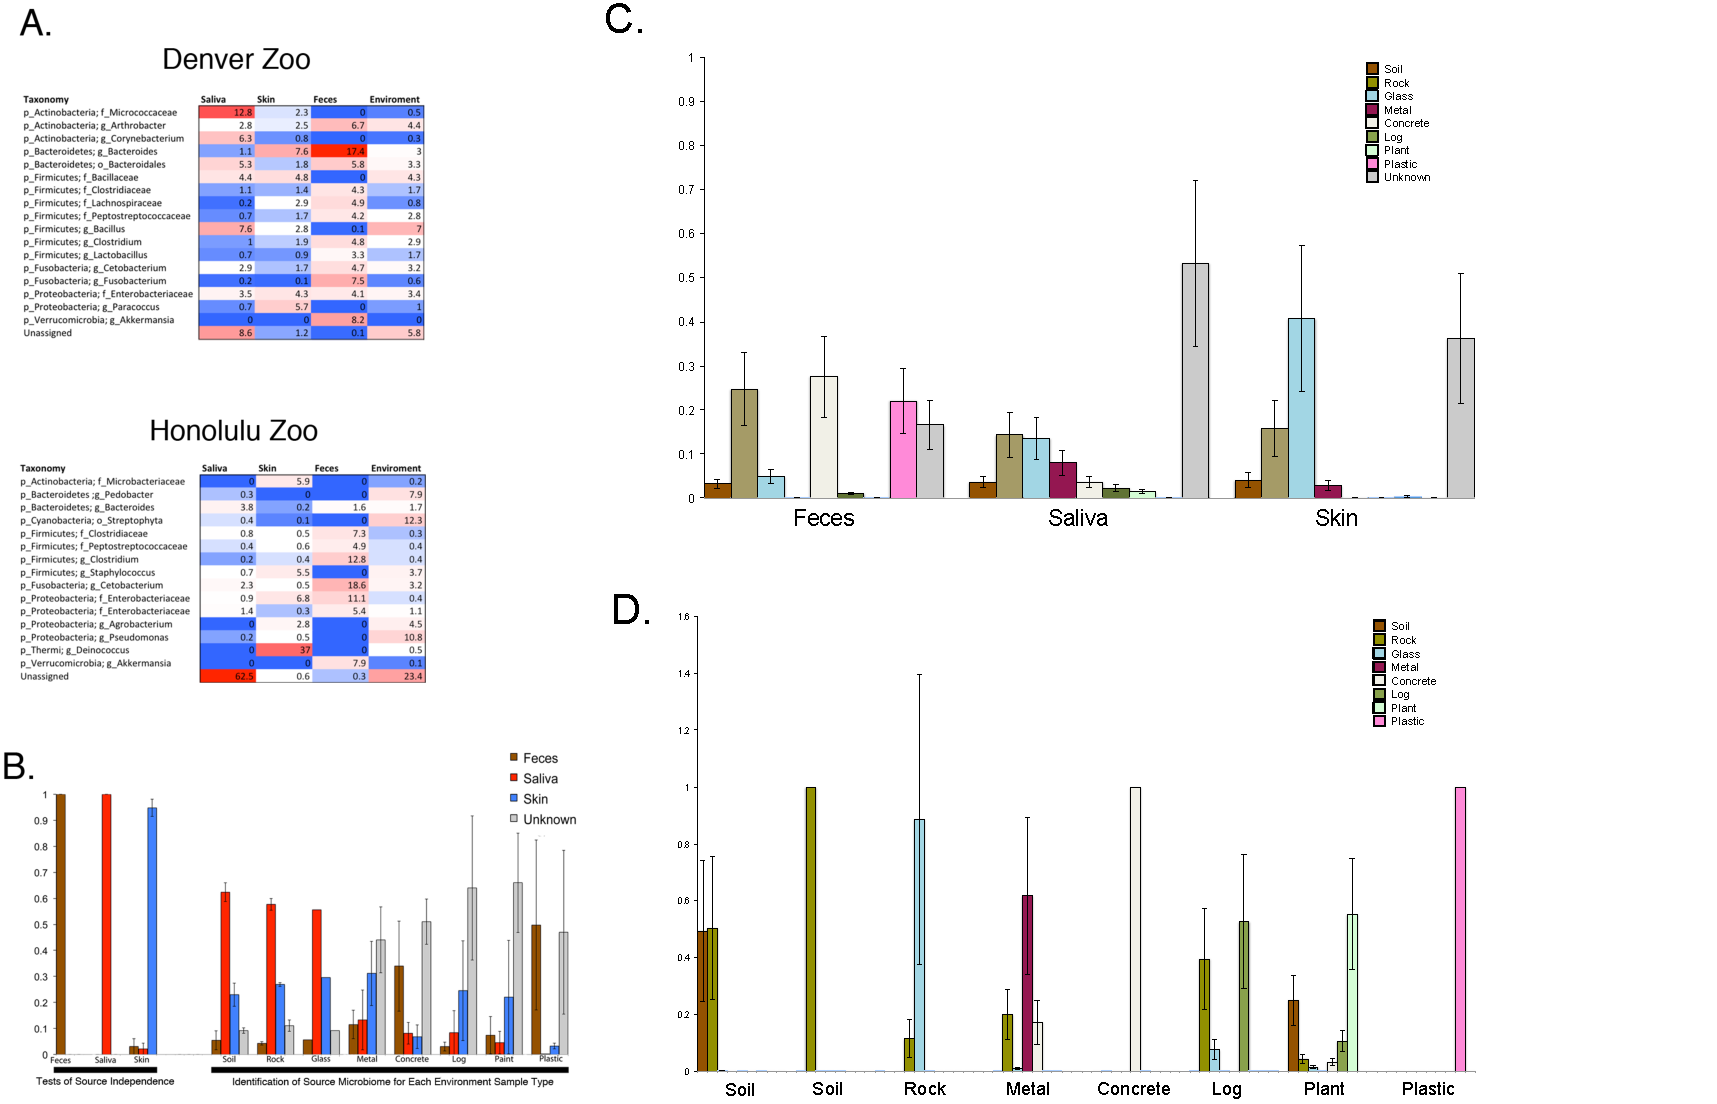
\includegraphics[width=1.15\columnwidth]{chapter_contributions_figures/KomodoSTest.pdf}
\caption[Taxonomy and SourceTracker results for the Komodo dataset]{\textbf{Taxonomy and SourceTracker results for the Komodo dataset.}
(A) Heat maps illustrate the percent abundances of the most abundant genera
(all \gls{otu}s taxonomically classified to the same genus were collapsed into
a single genus summary) present in saliva, skin, feces, and environmental (Env)
samples collected from the Denver and Honolulu zoos. The deepest taxonomic
classification achieved is listed for each genus. The heat map colors indicate
percent abundance (red [high abundance] to blue [low abundance]). (B) Komodo
dragon SourceTracker analysis reveals that the microbial communities of many
environmental sample types are sourced from skin, saliva, and feces rather than
unknown sources (i.e., not from Komodo dragon skin, saliva, or feces). Data are
plotted as the means $\pm$ standard errors of the means (error bars) of samples
from Denver and Honolulu zoo Komodo dragons. (C) SourceTracker analyses with
Komodo dragon fecal, salivary, and skin samples designated as sinks and environmental
samples designated as sources reveals that a variety of environmental sources,
rather than a single environmental source, contribute to the microbial communities
of Komodo dragon feces, saliva, and skin. Unknown sources (i.e., not the environments
sampled from the Komodo dragon enclosures) also contribute about 40\% or more of
the microbial community of saliva and skin samples (only 20\% of fecal samples).
(D) Independence tests reveal that about half of the environmental samples are not
independent from other environmental samples. Data are the means $\pm$ standard errors
of the means of Denver and Honolulu Komodo dragon and environmental samples.}
\label{KomodoST}
\end{figure}

To further assess host-environment microbiome sharing, in both closed/captive and
open/wild environments, we additionally performed SourceTracker analyses on two
previously published data sets—a wild amphibian skin-environment microbiome data set
\cite{Kueneman2014} and a human-pet-house microbiome data set \cite{Lax2014}—and
compared them to the Komodo dragon data set. As previously shown, humans and their
pets contribute a large amount of their microbiomes to their living environments
\cite{Lax2014}, similarly to the patterns we observed with captive Komodo dragons.
However, while Komodo dragon microbiome sources (skin, saliva, and feces) were
found to be distinct sources, we did not observe this level of source independence
when applying the SourceTracker independence test to the human/pet data set.

Host-environment microbiome sharing between amphibians and their living environment
was not as extensive as that observed among captive Komodo dragons and their
enclosures or humans and pets and their homes. More than 75\% of soil and sediment
microbial communities were obtained from unknown microbiome sources; however,
the identified “source” for 75\% of water microbial communities was amphibian skin
(Figure ~\ref{AmphibianST} A). Each source (here defined as individual amphibian
species) was highly independent from each other source (Figure ~\ref{AmphibianST} B).
Defining amphibian skin as a sink and environmental samples as sources, water was
identified as a major source of the microbes on the skin of most species; nevertheless,
at least 20\% of the microbial community on the skin of all species was contributed
by unknown sources (Figure ~\ref{AmphibianST} C). Soil, sediment, and water were
all confirmed to be independent sources (Figure ~\ref{AmphibianST} D).

\begin{figure}[htbp]
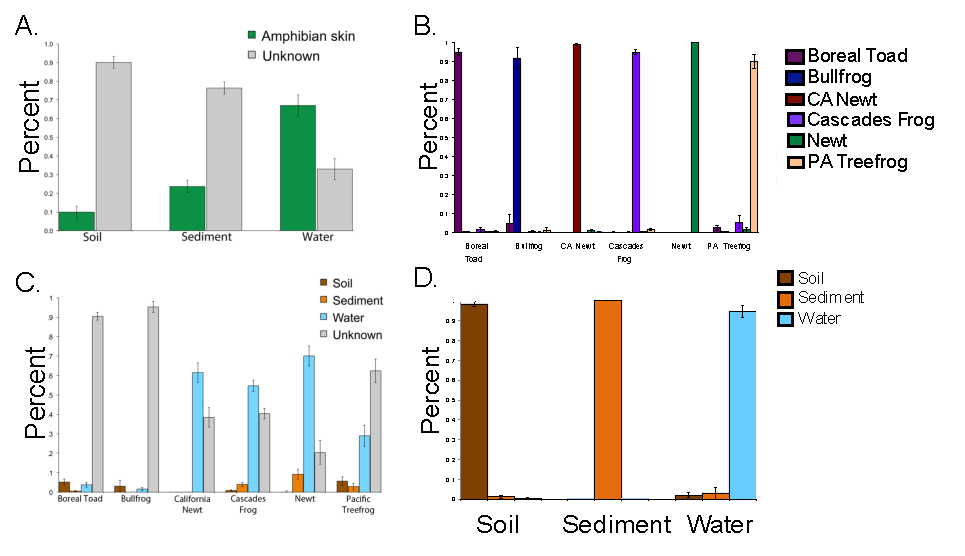
\includegraphics[width=\columnwidth]{chapter_contributions_figures/AmphibiansST.pdf}
\caption[SourceTracker results for the amphibians dataset]{\textbf{SourceTracker results for the amphibians dataset.}
(A) Amphibian SourceTracker analysis reveals that water is the only sample type
that obtains a notable amount of its microbial community from amphibian skin; unknown sources
(i.e., not amphibian skin) are the main microbiome contributors to soil and sediment.
(B) Independence tests reveal that amphibian skin is independently specific to species.
(C) Designating environment the source and amphibian skin the sink reveals that water
is the only environmental type that contributes largely to the microbial communities
on amphibian skin, with unknown sources also largely contributing to the amphibian
skin microbiome. (D) Independence tests reveal that each environment type is also
independent from each other environment type. Data are the means $\pm$ standard
errors of the means.}
\label{AmphibianST}
\end{figure}

\subsection{A communal catalogue reveals Earth's multiscale microbial diversity}\label{subsection_emp}

The following material has been adapted from the original publication in
\textsl{Nature, 2017}. As a contributor to this manuscript, I quality filtered the
97 independent studies included in the manuscript, generated the \gls{otu}-based
closed and open reference tables and the open reference phylogenetic tree and provided
scripts to reproduce those steps.

The \gls{emp} was founded in 2010 to sample the Earth's microbial communities at an
unprecedented scale in order to advance our understanding of the organizing
biogeographic principles that govern microbial community structure
\cite{Gilbert2010, Gilbert2014, Thompson2017}. The \gls{emp} asked the global scientific
community for environmental samples and associated metadata spanning diverse
environments and capturing spatial, temporal, and/or physicochemical covariation.
The first 27,751 samples from 97 independent studies represent diverse environment
types (Figure ~\ref{EMProvenance} A), geographies (Figure ~\ref{EMProvenance} B),
and chemistries. The \gls{emp} encompasses studies of bacterial, archaeal, and
eukaryotic microbial diversity. The analysis here focuses exclusively on the
bacterial and archaeal components of the overall database (for concision, use of
‘microbial’ will hereafter refer to bacteria and archaea only). Associated metadata
included environment type, location information, host taxonomy (if relevant), and
physicochemical measurements. Physicochemical measurements were made in situ at
the time of sampling. Investigators were encouraged to measure temperature and
pH at minimum. Salinity, oxygen, and inorganic nutrients were measured when possible,
and investigators collected additional metadata pertinent to their particular investigations.

\begin{figure}[htbp]
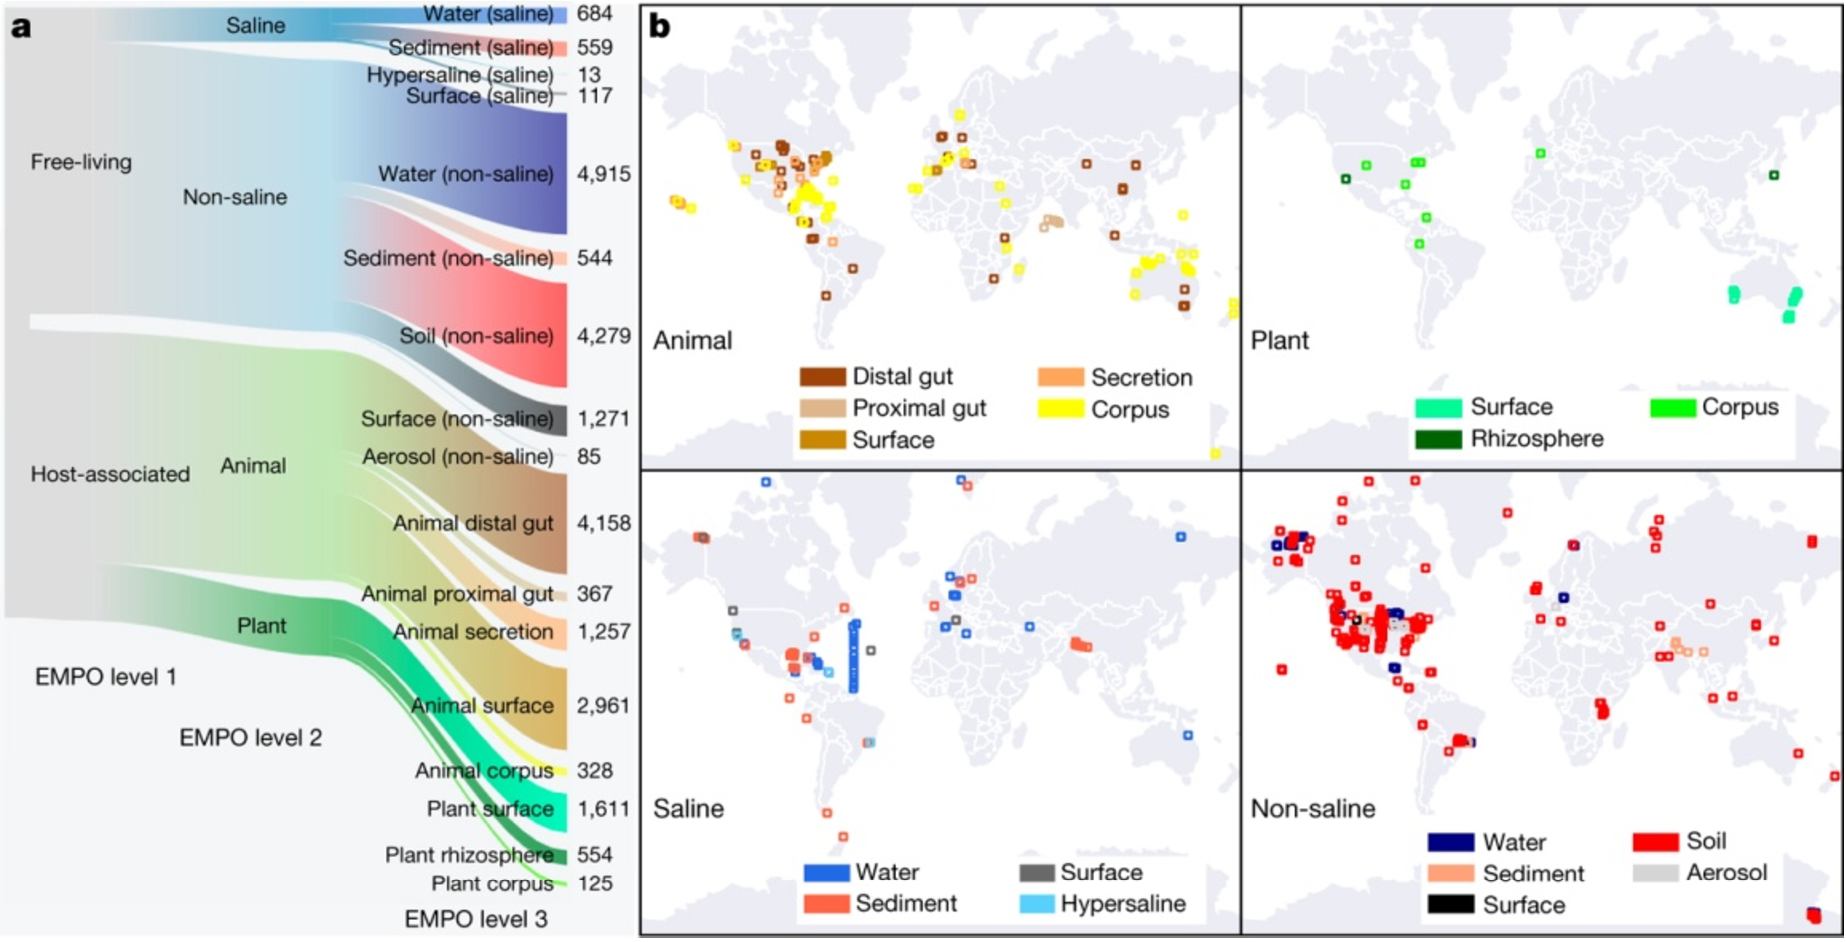
\includegraphics[width=\columnwidth]{chapter_contributions_figures/EMProvenance.pdf}
\caption[Environment type and provenance of samples]{\textbf{Environment type and provenance of samples.}
(A) The \gls{empo} classifies microbial environments (level 3) as free-living or
host-associated (level 1) and saline or non-saline (if free-living) or animal
or plant (if host-associated) (level 2). The number out of 23,828 samples in the
QC-filtered subset in each environment is provided. \gls{empo} is described with examples
at http://www.earthmicrobiome.org/protocols-and-standards/empo. (B) Global scope of
sample provenance: samples come from 7 continents, 43 countries, 21 biomes (\gls{envo}),
92 environmental features (\gls{envo}), and 17 environments (\gls{empo}).}
\label{EMProvenance}
\end{figure}

Beyond measured physical covariates, the breadth of environments in the \gls{emp}
catalogue allows a detailed exploration of how microbial diversity is distributed
across environments. Diversity among communities (beta-diversity) is driven by
turnover (replacement of taxa) and nestedness (gain or loss of taxa resulting in
differences in richness) \cite{Carvalho2013}. If turnover dominates, then
disparate communities will harbour unique taxa. If nestedness dominates, then
communities with fewer taxa will be subsets of communities with more taxa. We
tested for nestedness using a 2,000-sample subset with even representation across
environments and studies. Given the contrasting environments and geographic separation
among the many studies in the \gls{emp}, we expected different environments to
contain unique sets of taxa and to show little nestedness. However, we found that
communities across environments were significantly nested (Figure ~\ref{EMPNestedness} A, B; P < 0.05)
in comparison to null models (Figure ~\ref{EMPNestedness} C), accounting for the
observed patterns of richness. At coarse taxonomic levels, an average of 84\% of phyla,
73\% of classes, and 58\% of orders that occurred in less diverse samples also
occurred in more diverse samples. These patterns could have resulted from several
mechanisms, including ordered extinctions \cite{Sonnenburg2016} and the filtering
of complex communities over time \cite{Atmar1993}, differential dispersal
abilities \cite{Lomolino1996} and cascading source–sink colonization processes
that assemble nested subsets from more complex communities, or by the tendency
of larger habitat patches to support more rare taxa with lower prevalence \cite{Gaston2000}.
Notably, finer taxonomic groupings showed less nestedness (Figure ~\ref{EMPNestedness} C),
indicating that the processes that underlie nested patterns of turnover are
likely to reflect conserved aspects of microbial biology, and not to result from
the interplay of diversification and dispersal on short timescales.

\begin{figure}[htbp]
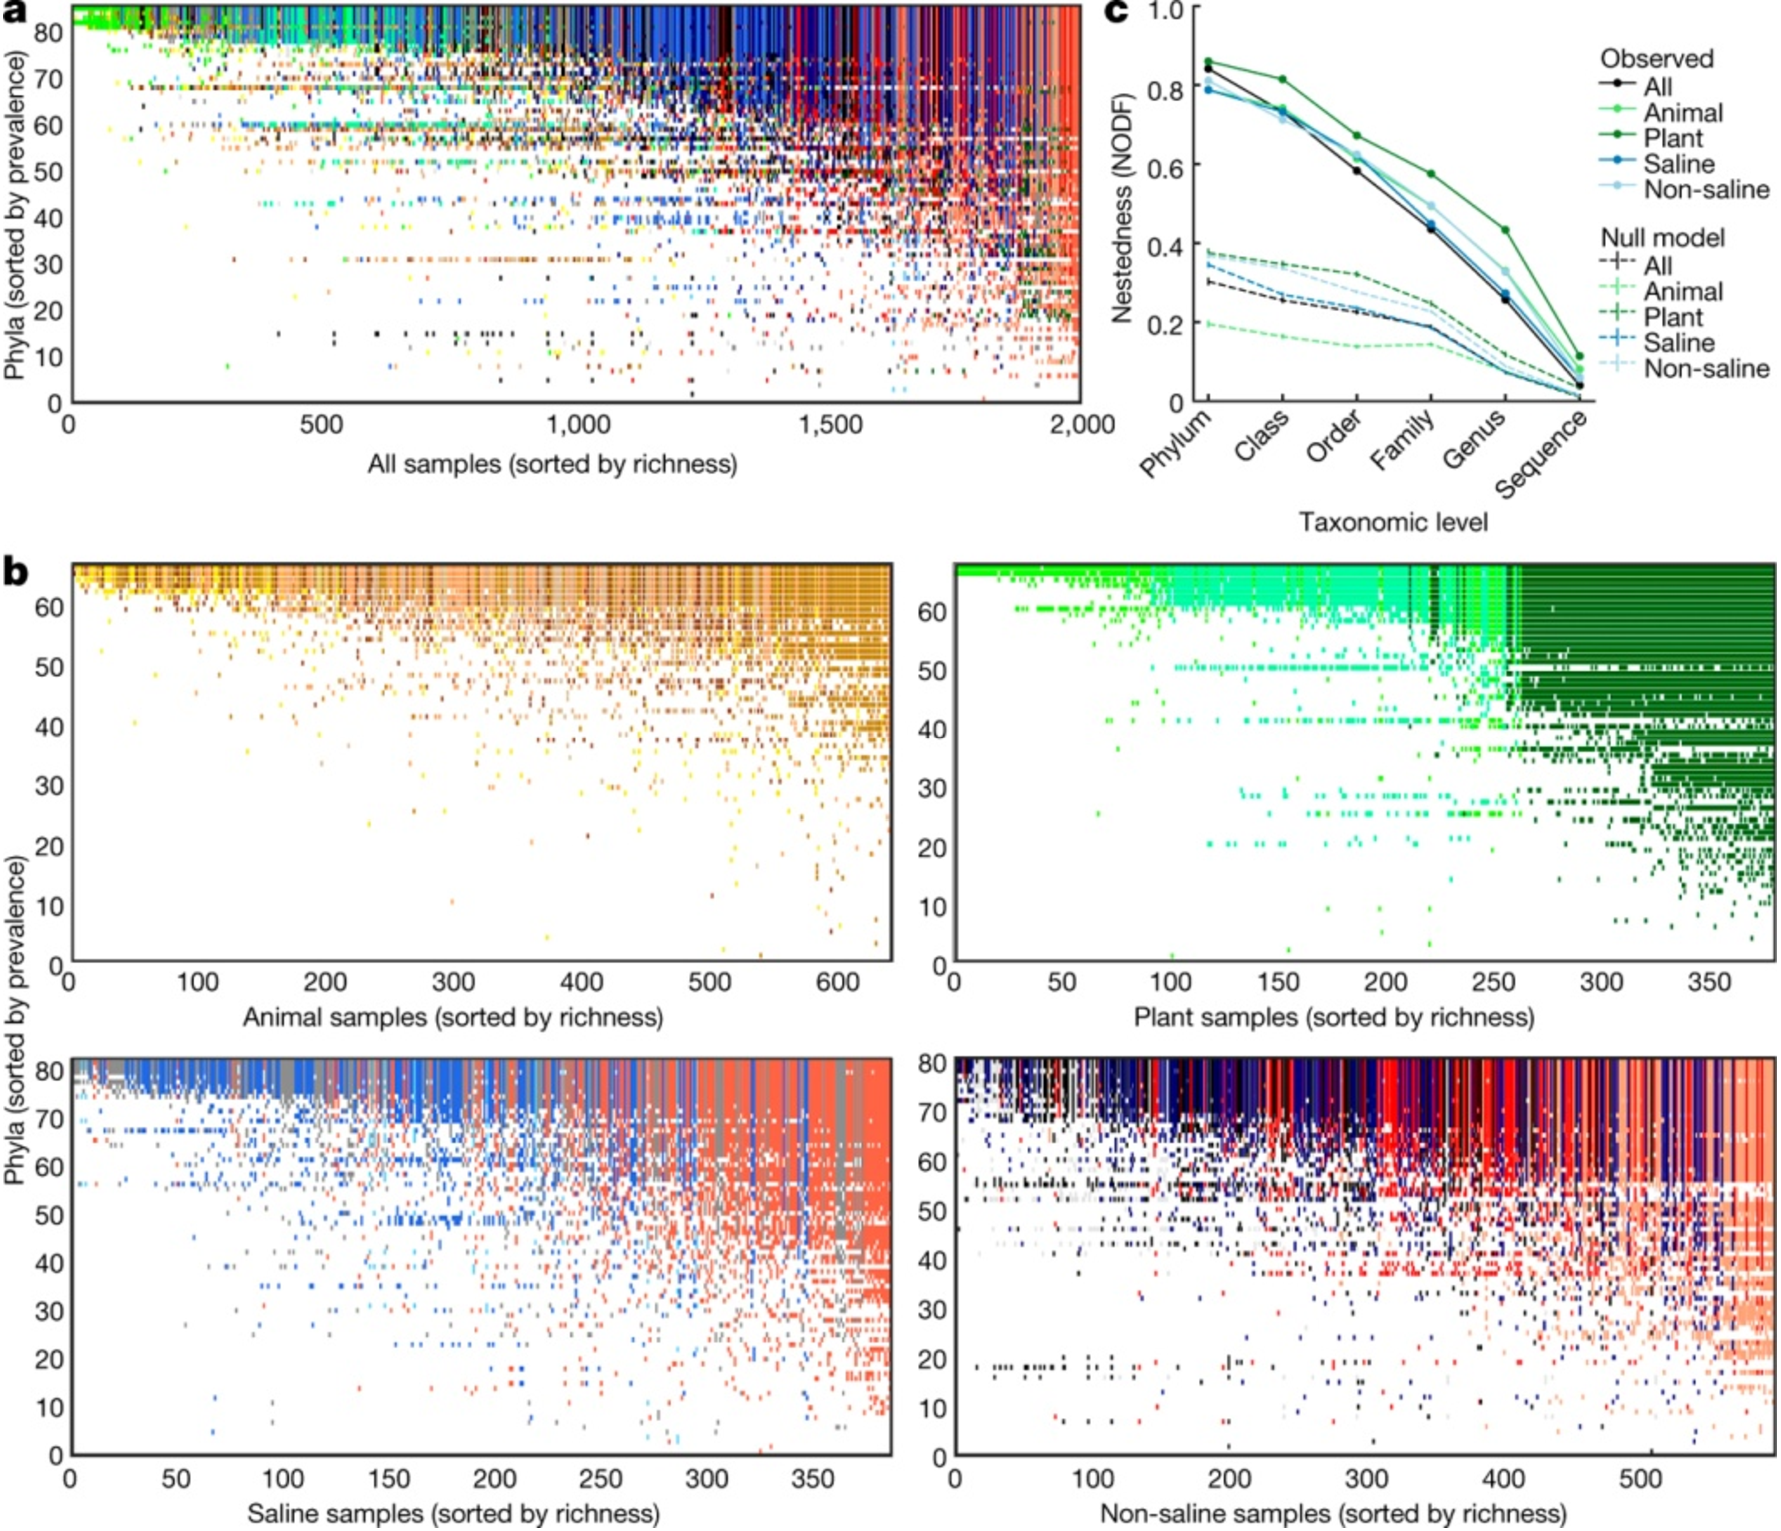
\includegraphics[width=\columnwidth]{chapter_contributions_figures/EMPNestedness.pdf}
\caption[Nestedness of community composition]{\textbf{Nestedness of community composition.}
(A) Presence–absence of phyla across samples, with phyla (rows) sorted by prevalence and samples
(columns) sorted by richness. Shown is a subset of the \gls{emp} consisting of n = 2,000
biologically independent samples with even representation across environments and studies.
With increasing sample richness (left to right), phyla tended to be gained but not lost
(P < 0.0001 versus null model; NODF (nestedness measure based on overlap and decreasing fills)
statistic and 95\% confidence interval = 0.841 $\pm$ 0.018). (B) As in A but separated into
non-saline, saline, animal, and plant environments (P < 0.0001, respective NODF = 0.811
$\pm$ 0.013, 0.787 $\pm$ 0.015, 0.788 $\pm$ 0.018 and 0.860 $\pm$ 0.021). (C) Nestedness as
a function of taxonomic level, from phylum to tag sequence, across all samples and within
environment types. Also shown are median null model NODF scores ($\pm$ s.d.).
NODF measures the average fraction of taxa from less diverse communities that occur in
more diverse communities. All environments at all taxonomic levels were more nested than
expected randomly, with nestedness higher at higher taxonomic levels (for example, phyla).}
\label{EMPNestedness}
\end{figure}

\subsection{American Gut: An open platform for citizen-science microbiome research}\label{subsection_ag}
The following material has been adapted from the original publication submitted in
\textsl{Science, 2018}. As a contributor to this manuscript, I generated the per
participant results, provided support maintaining the software and reviewed drafts
of the manuscript.

We therefore launched the \gls{agp} \footnote{\url{http://americangut.org}}, now the
largest crowdfunded and crowdsourced microbiome citizen-science project to date,
with the goal to discover the kinds of microbes and microbiomes "in the wild.”
Our project informs participants about their own microbiomes by providing them with
a standard report that places them in context of the full AGP and Human Microbiome
Project (HMP) datasets, and provides a broad set of resources to support research
about the human microbiome, including an online course. Unlike many other large
microbiome studies, the AGP deposits all de-identified data into the public domain
on an ongoing basis without access restrictions. This reference database has allowed
us to characterize the diversity of the industrialized human gut microbiome at an
unprecedented scale, to explore novel relationships with health, lifestyle, and
dietary factors, and to establish the AGP resource and infrastructure as a living
platform for discovery (e.g., through targeted sub-populations and through the
application of multi-omics techniques).

Key variables that we found to have the greatest effects on the composition of gut
microbes - plant consumption, antibiotic use, and even age - are in flux in the global
population. Our lifespans are increasing, we are traveling more, our diets are
becoming homogenized, and we are consuming more antibiotics. In each case, these
trends are likely to favor more homogenization and less diverse gut microbes.
Ongoing efforts, such as the AGP, will allow researchers to document and potentially
mitigate the effects of such change. They will also afford insights into our past
through collections from more diverse subpopulations, which will allow us to better
understand the context of our choices in the future.

A unique aspect of the AGP is the open community process of assembling the Research
Network and analyzing these data. Because participants fund the project, no funding
agency mandates restrictions on data analysis to a specific group of investigators.
Thus, these data are released into the International Nucleotide Sequence Database
Collaboration (INSDC) (and GNPS for metabolomics data) as soon as initial quality
control and anonymization steps have been applied. Analysis details are shared
through a public forum \footnote{GitHub, \url{https://github.com/knightlab-analyses/american-gut-analyses}}.
Scientific contributions to the project were made through a geographically diverse
Research Network represented herein as the American Gut Consortium (including explicitly
named authors). This network was established prior to project launch and has continued
to grow over time. The analyses described were performed through an open contribution
model in which pre-computed forms of these data were publicly provided with encouragement
to the American Gut Consortium to explore the dataset. This model allows the project to
use a “living analysis” approach, embracing new researchers and analytical tools on an
ongoing basis (e.g., Qiita and Global Natural Products Social Molecular Networking (GNPS)).
Additionally, because the AGP is a subproject of the Earth Microbiome Project (EMP) \cite{Thompson2017}),
all samples were processed using the publicly available and widely used EMP 16S rRNA gene
amplification, sequencing, and data analysis protocols to facilitate meta-analyses. For
example, we combined the AGP with fecal samples collected from a fecal transplant
study and an infant microbiome time series, the latter using different DNA sequencing
technology, to highlight how this context can provide insight.


\subsection{Correcting for microbial blooms in fecal samples during room-temperature shipping}\label{subsection_bloom}
The following material has been adapted from the original publication in
\textsl{mSystems, 2016}. As a contributor to this manuscript, I was involved in
the discussion for establishing the criteria to choose blooming bacteria, provided
input on the figures design and reviewed drafts of the manuscript.

The use of sterile swabs is a convenient way to collect samples for microbiome studies,
but in some cases, it is not feasible to immediately freeze or utilize a preservative.
For example, the \gls{agp} allows members of the general public to send samples for 16S
\gls{rrna} gene amplicon sequencing through domestic post without a preservative.
This is because proven preservation methods can be cumbersome, dangerous, expensive,
or sample type specific, complicating participation in microbiome citizen science.
Although some studies have demonstrated that the effects of room-temperature storage
are secondary to physiologically relevant differences between comparison groups
\cite{Song2016, Sinha2016, Lauber2010}, certain bacterial taxa,
particularly those in the class \emph{Gammaproteobacteria}, grow well at room temperature.
This is problematic, as some \emph{Gammaproteobacteria} species have been associated
with disease, such as \gls{ibd} \cite{Gevers2014}. Therefore, to identify meaningful
patterns in microbiome studies that do not utilize sample preservation, it is crucial
to remove at high specificity the taxa that thrive at room temperature (i.e., “blooming” bacteria).

Without filtering candidate blooms, there were notable differences (as observed using Bray-Curtis
\gls{pcoa}) between \gls{agp} fecal samples and the fresh-frozen fecal samples;
filtering the bloom sequences from all samples removed these differences (Figure ~\ref{bloomFig} A versus B).
In the \gls{pcoa} space corresponding to the data determined without filtering, the primary
separation is explained by the presence of a large percentage of bloom sequences (Figure ~\ref{bloomFig} A);
the sizes of the spheres are scaled by the percentage of bloom sequences in the respective sample.
Following the removal of the blooms, this dominant effect was abolished and samples with high levels of
blooms clustered with samples from the other studies (Figure ~\ref{bloomFig} B). Similar results were observed
in assessing class-level taxonomy abundances (Figure ~\ref{bloomFig} C versus D): prior to filtering,
a high relative abundance of \emph{Gammaproteobacteria} (27\%) was present in the \gls{agp} samples
compared to the fresh-frozen samples (1.5\% to 3.5\%), while the \gls{agp} profile seen after filtering
more closely resembled that of the fresh-frozen samples. Importantly, applying the filter minimally
changed the taxonomic profiles of fresh-frozen samples (Figure ~\ref{bloomFig} D). The filtering
procedure is available in a Jupyter Notebook \cite{Perez2007} at https://github.com/knightlab-analyses/bloom-analyses.

There is a balance between type 1 and type 2 errors that must be considered in applying this filter.
The cost of removing a sequence is that it becomes “invisible” in the analysis, and it is possible
that real sequences are lost. Conversely, retaining a bloom sequence increases noise caused by shipment
conditions, which can artificially alter biological conclusions. Therefore, a balance between loss of data
and inaccurate, noisy data must be obtained. To select an appropriate number of blooming bacterial
sequences to subtract from the \gls{agp} data set to maximize the amount of data retained while
reducing inaccuracies caused by blooms, we tested the effect of nested filtering levels on the ability
to detect the well-known effect of age on alpha diversity \cite{Yatsunenko2012, Koenig2011}.
As can be seen in Figure ~\ref{bloomFig} E and F,
this effect was undetected by a Kruskal-Wallis test when none of the candidate blooms were removed.
However, filtering the top four candidate blooms restored the ability to detect a significant
difference in diversity by age. Critically, the identification of the bloom sOTUs was done
independently of this positive control. For analysis of the \gls{agp} cohort, we recommend
removal of the sequences of the top 10 candidate blooming bacterial taxa, as this maximizes the expected
age effect (Figure ~\ref{bloomFig} E). Different studies may need to remove a different subset of
bloom sequences, as retaining some of these sequences might be critical, depending on the study
characteristics. With meta-analysis, if this filter is applied, it must be applied identically to
all samples represented to avoid introduction of a systematic bias.

\begin{figure}[htbp]
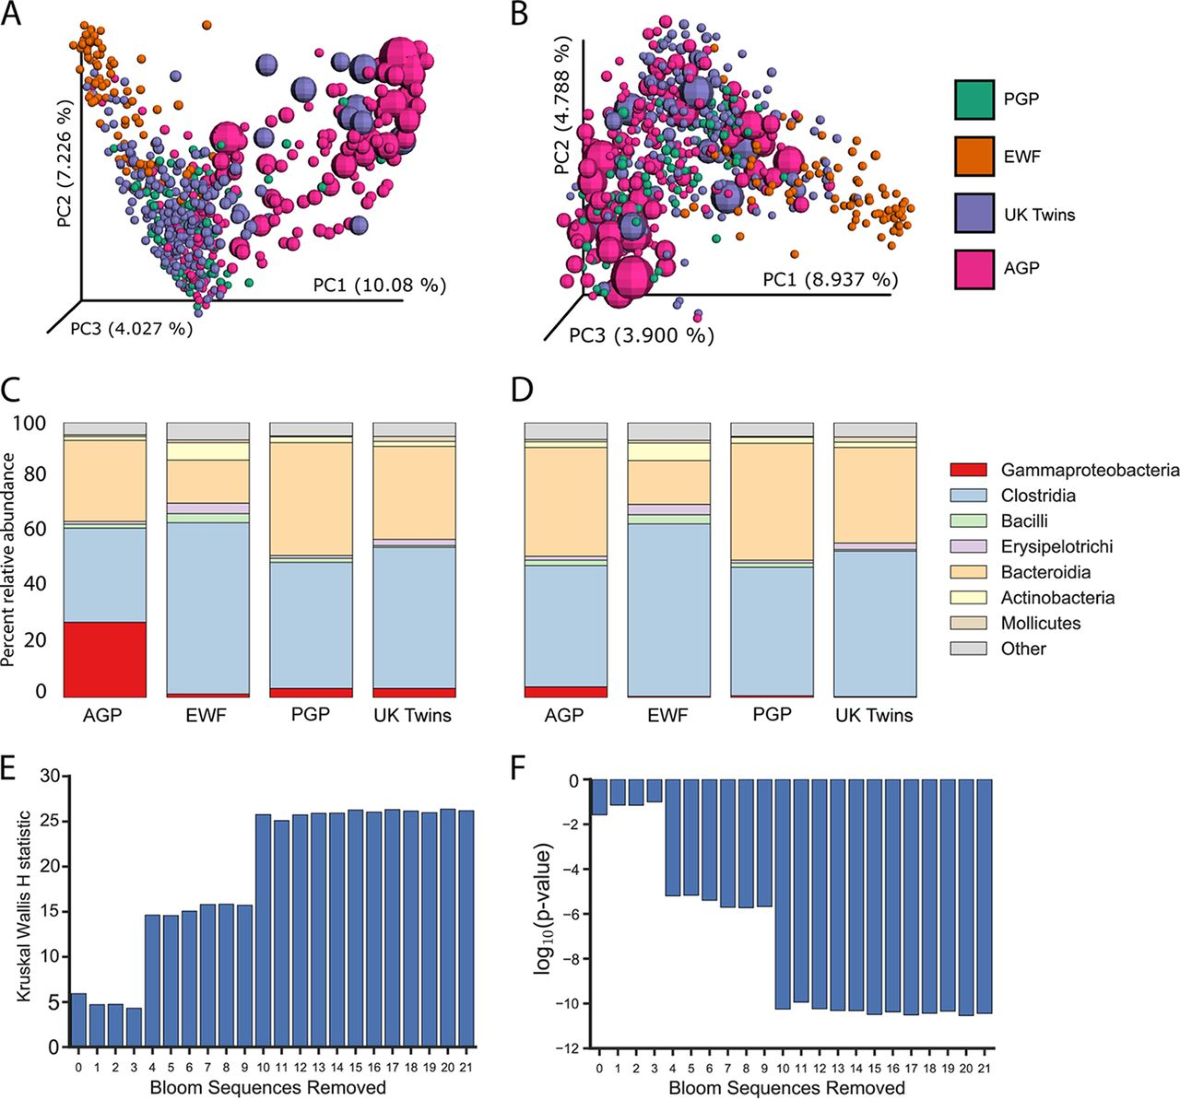
\includegraphics[width=\columnwidth]{chapter_contributions_figures/bloom.pdf}
\caption[Effect of bloom filtering on American Gut data]{\textbf{Effect of bloom filtering on American Gut data.}
(A and B) \gls{pcoa} of Bray-Curtis distances from a random subset of 200 American Gut Project samples (colored pink)
compared to 3 studies containing fresh-frozen fecal samples: Personal Genome Project (colored green);
whole-grain feces \cite{Vitaglione2015} (colored orange); and UK Twins \cite{Goodrich2017} (colored purple), respectively.
The \gls{pcoa} data shown represent results obtained before (A) and after (B) applying the
filter for blooms to all samples. The size of a sphere is scaled by the amount of
candidate bloom bacteria in a sample prior to filtering. (C and D) Mean taxonomy distribution for the
same studies before (C) and after (D) filtering for blooms. (E and F) The well-known effect of age on
alpha diversity and how the effect is observed only after the removal of bloom reads.
The Kruskal-Wallis test statistic (E) and corresponding –log(P value) (F) are shown for
different numbers of bacteria used for the filtering before applying the test. A value of 0 on the
x axis indicates no filtering. The x axis is ordered by decreasing severity score of the bloom where bloom
1 represents greater severity than bloom 2, and each point on the x axis includes the prior blooms
(e.g., position 5 includes bloom sOTUs 1 through 5).}
\label{bloomFig}
\end{figure}
